%-*-latex-*-
\sectionthree{Queue}
\begin{python0}
from solutions import *; clear()
\end{python0}

A queue (see CISS240/245) is an ADT where you can put things into the container
and you can take things out of it.
The operation of putting a value into a queue is called enqueue
and the operation of taking a value out of a queue is called dequeue.
Like the stack, it's self-organizing: you don't have to tell the
queue where to put a value and you don't have to tell the queue
which one to remove.

Suppose this is a queue:


\begin{longtable}{|r||r|r|r|r|r|}
\hline 
         & $w_1$ & $w_2$ & $w_3$ & $w_4$ & $\ldots$ \\ \hline \hline 
$M_1$    &       &       &       &       &          \\ \hline 
$M_2$    &       &       &       &       &          \\ \hline 
$M_3$    &       &       &       &       &          \\ \hline 
$M_4$    &       &       &       &       &          \\ \hline 
$\ldots$ &       &       &       &       &          \\ \hline 
\end{longtable}
        


A queue has a front and a back.
Let's say for the above diagram the value 1 is the front and the 3 is the back.
If I enqueue with 7, the queue becomes:


\begin{longtable}{|r||r|r|r|r|r|}
\hline 
         & $w_1$ & $w_2$ & $w_3$ & $w_4$ & $\ldots$ \\ \hline \hline 
$M_1$    & 0     & 0     & 1     & 0     & ...      \\ \hline 
$M_2$    & 1     & 0     & 1     & 1     & ...      \\ \hline 
$M_3$    & 0     & 1     & 1     & 1     & ...      \\ \hline 
$M_4$    & 1     & 0     & 1     & 1     & ...      \\ \hline 
$\ldots$ &       &       &       &       &          \\ \hline 
\end{longtable}
        


If I dequeue, the 1 is removed (frequently returned) and the queue
becomes

\begin{center}
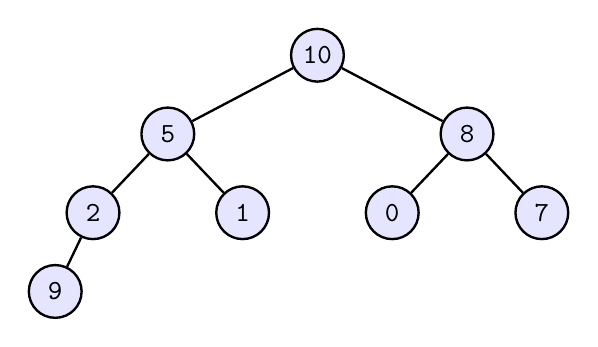
\begin{tikzpicture}

\fill[blue!10] (0.0, 0.0) circle (0.35);
\node [line width=0.03cm,black,minimum size=0.6699999999999999cm,draw,circle] at (0.0,0.0)(10){};\draw (0.0, 0.0) node[color=black] {\texttt{10}};
\fill[blue!10] (-1.9, -1.0) circle (0.35);
\node [line width=0.03cm,black,minimum size=0.6699999999999999cm,draw,circle] at (-1.9,-1.0)(5){};\draw (-1.9, -1.0) node[color=black] {\texttt{5}};
\fill[blue!10] (1.9, -1.0) circle (0.35);
\node [line width=0.03cm,black,minimum size=0.6699999999999999cm,draw,circle] at (1.9,-1.0)(8){};\draw (1.9, -1.0) node[color=black] {\texttt{8}};
\fill[blue!10] (-2.85, -2.0) circle (0.35);
\node [line width=0.03cm,black,minimum size=0.6699999999999999cm,draw,circle] at (-2.85,-2.0)(2){};\draw (-2.85, -2.0) node[color=black] {\texttt{2}};
\fill[blue!10] (-0.95, -2.0) circle (0.35);
\node [line width=0.03cm,black,minimum size=0.6699999999999999cm,draw,circle] at (-0.95,-2.0)(1){};\draw (-0.95, -2.0) node[color=black] {\texttt{1}};
\fill[blue!10] (0.95, -2.0) circle (0.35);
\node [line width=0.03cm,black,minimum size=0.6699999999999999cm,draw,circle] at (0.95,-2.0)(0){};\draw (0.95, -2.0) node[color=black] {\texttt{0}};
\fill[blue!10] (2.85, -2.0) circle (0.35);
\node [line width=0.03cm,black,minimum size=0.6699999999999999cm,draw,circle] at (2.85,-2.0)(7){};\draw (2.85, -2.0) node[color=black] {\texttt{7}};
\fill[blue!10] (-3.33, -3.0) circle (0.35);
\node [line width=0.03cm,black,minimum size=0.6699999999999999cm,draw,circle] at (-3.33,-3.0)(9){};\draw (-3.33, -3.0) node[color=black] {\texttt{9}};\draw[line width=0.03cm,black] (10) to  (5);
\draw[line width=0.03cm,black] (10) to  (8);
\draw[line width=0.03cm,black] (5) to  (2);
\draw[line width=0.03cm,black] (5) to  (1);
\draw[line width=0.03cm,black] (8) to  (0);
\draw[line width=0.03cm,black] (8) to  (7);
\draw[line width=0.03cm,black] (2) to  (9);
\end{tikzpicture}

\end{center}



Note that the value removed is the value that was in the queue the
longest.
So we say that a queue is a
\defterm{first-in-first-out}\tinysidebar{first-in-first-out\\ FIFO}\index{first-in-first-out},
\defterm{FIFO}\index{FIFO},
data structure.

You see queues everywhere:
a network router processes messages that are stored in a queue.
A webserver processes requests that are stored in a queue.
The OS running your laptop will run processes that are stored in a queue.
I/O requests are also stored in queues.
Etc.

Note that since you have to operate a queue on both ends,
you should use a doubly linked list and not a singly linked list.
(An array implementation is possible if the maximum length of the
queue is small and fixed.)

Frequently, jobs entering a queue has a priority number
that allows the job to jump ahead.
For instance the following is a queue of jobs and the
numbers are the priority numbers where low means high priority:


\begin{center}
\begin{tikzpicture}[>=triangle 60,shorten >=0.5pt,node distance=2cm,auto,initial text=, double distance=2pt]
\node[state,initial] (A) at (  0,  0) {$\{q_0\}$};
\node[state] (B) at (  3,  0) {$\{\}$};

\path[->]
(A) edge [bend left=0,pos=0.5,above] node {$a,b$} (B)
(B) edge [loop above] node {$a,b$} ()

;
\end{tikzpicture}
\end{center}
    


So if I enqueue 5, the 5 will enter the queue at the end
but will jump ahead of the job with priority 7,
jump ovrer the jobn with priority 6, but will not jump ahead of the
job with priorityt 5 that was already there:


\begin{center}
\begin{tikzpicture}[>=triangle 60,shorten >=0.5pt,node distance=2cm,auto,initial text=, double distance=2pt]
\node[state,initial] (A) at (  0,  0) {};

\path[->]
(A) edge [loop above] node {$a,b$} ()

;
\end{tikzpicture}
\end{center}
    


Such things are called priority queues.
We'll come back to this later when we look at heaps.


\begin{ex}
  \begin{tightlist}
    \li If you use an array to implement a queue, what is the
    runtime of enqueue and dequeue?
    \li If you use a singly linked list to implement a queue, what is the
    runtime of enqueue nad dequeue? (Remember that in this case
    you have to say where is the front and where is the end of the queue
    with respect to the list.)
    \li If you use a doubly linked list to implement queue, what is the
    runtime of enqueue nad dequeue? 
  \end{tightlist}
  \qed
\end{ex}

\begin{ex}
  \begin{tightlist}
    \li If you use an array to implement a priority queue, what is the
    runtime of enqueue and dequeue?
    \li If you use a singly linked list to implement a priority
    queue, what is the
    runtime of enqueue nad dequeue? (Remember that in this case
    you have to say where is the front and where is the end of the queue
    with respect to the list.)
    \li If you use a doubly linked list to implement a priority
    queue, what is the
    runtime of enqueue nad dequeue? 
  \end{tightlist}
  \qed
\end{ex}
